%-----------------------------------------------------------------
%	ALTERNATIVE IMPLEMENTATIONS
%	!TEX root = ./../main.tex
%-----------------------------------------------------------------



\section{Alternative Controlling Methods}

We have used alternative methods that do not use control theory in order to make the trailer follow the path that we want. These methods focus on different heuristics to determine which $\delta$ we have to choose in order to go through the desired path. The first method thinks on a function to optimise in order to be as close as possible to the desired path and as close as possible to the critical point $\phi = 0$. The second one aims to replicate the strategy of expert trailer drivers that have a lot of experience in our problem.\\

\subsection{Optimisation-based control}

Using the model derived in \cref{kinem}, we aim to move our trailer in a straight path. Of course, our straight path will start with an angle $\phi \neq 0$, which tries to resemble a situation where we are trying to go backwards but the trailer starts to bend due to some imperfection of the ground/wheels.\\

We will assume, without loss of generality, that the centre of mass of our car starts at the origin. As we want the car to go straight, we will make the car go backwards in the $x$ axis, and the car will start aligned with this axis. On the other hand, the trailer will not start aligned with the $x$ axis (if not, the solution would be trivial, setting $\delta = 0$ the whole time would solve the problem). Our aim is to go through the $x$ axis during a quantity of time $T$. However, what does going through the $x$ axis mean?
We will set a tolerance $\Delta y$, and if at time $T$ the trailer is at a distance from the $x$ axis lower than $\Delta y$, we will take it a success. In mathematical terms, we have to decide a function $\delta(t)$, for $0\leq t \leq T$, such that $\abs{y(T)} < \Delta y$ and $\abs{\phi} < \phi_{crit}$, where $\phi_{crit}$ is the critical jackknifing angle.\\

To find the \textit{steering function} $\delta(t)$, we will use a brute force method. We will split the interval $[0, T]$ into $n$ interval times of length $T/n$. At the beginning of each interval, we will choose which is the $\delta$ that puts the trailer in the best possible configuration at the end of the interval. We will simulate the trajectory of the whole system in order to decide how good is a choice of $\delta$. In addition, we have to determine when is a configuration better than another one. To do this, we have chosen a cost function. The cost function that we have chosen depends on the angle $\phi$ and the distance from the $x$ axis, $\abs{y}$. We have taken:
\begin{align}
    \operatorname{cost}_{\alpha}(y, \phi) = y^2+\alpha\phi^2 
\end{align}
The cost function defined above depends on a parameter, $\alpha$. The higher $\alpha$ is, the more we are interested in keeping the trailer aligned. The lower $\alpha$ is, the more we are interested in keeping the car on the path regardless of the trailer. Then, $\alpha$ is a parameter that needs to be tuned in every different geometrical configuration. \\

Now that we have our cost function defined, our method to find the steering function $\delta(t)$ works as follows: for each of the time intervals that we have divided our time into, at the beginning of the interval we choose the $\delta$ that minimises $\operatorname{cost}_{\alpha}$ at the end of the interval. The way to find the optimal $\delta$ is by means of brute force: We search in a grid of angles in the interval $[-\delta_{max}, \delta_{max}]$ and number of elements $n_{\delta}$. With this method, the output function $\delta(t)$ is a piecewise function that at every time interval has a constant value.\\

One of the main drawbacks of the method is that, given a time $T$, the method depends on three parameters that we do not know which value they should have a priori: $n$, $n_\delta$ and  $\alpha$. One could argue that, the higher the $n$, the more chances that the method can find the solution. However, this is far from the truth. The main problem is that method tries to optimise the configuration of the system at the next time step: however, this does not in principle guarantee that this configuration will be optimal after that time step. For this reason, having a very large $n$ can be considered very elitist, thus not allowing us to find the proper steering function. These kind of elitist searches are usually known as greedy algorithms.\\

We have implemented the previous method in $C$, using the analytical expressions for the circular paths of the points in the car and using a Runge--Kutta--Fellberg 78 method to integrate the differential equation for $\phi$. We have used sensible data for the length and width of each of the elements of the system.  Our aim would be to keep the system going straight for a given amount of time $T$. When $T$ is large enough ($T\approx 10$ seconds), the system is very hard to be controlled in the whole interval. We have tried many values of $\alpha$, $n$ and $n_\delta$, but they all fail when given a sufficiently large amount of time $T$.\\


We think that this method does not work due to the fact that the method only focuses on optimising the next time step. This is a main drawback, as not only it forgets about time steps that follow the next one, but it may also be that optimising the next time step is bad for the long run. In terms of optimisation, we can say that we are constantly being elitist, and this is usually not the best strategy when we want to optimise complicated functions. For this reason, the next method is a little bit more exploratory, that is, it does not always look at the best solution in its neighbourhood, but in the long run it performs better.\\

% \subsection{Experienced control}
\subsection{Steering-based control}
In this section we describe the method to get the trailer from one point to another by using steering strategies that reassemble the ones used by experienced drivers.\\

The method is made up of iteratively-repeated steering steps that we have defined as a \textit{manoeuvre}. A \textit{manoeuvre} consists in two steps: the first one, to bend the trailer into the right direction, and the second one, to move the car towards the desired end.\\

We will call the first part of the \textit{manoeuvre} \emph{trailer facing}. The way to perform \emph{trailer facing} is the following. Assume that if you had to go from the beginning point to the final point \textit{without} a trailer you would have to take $\delta > 0$ to go upwards. In this case, the trailer would quickly face the opposite direction, it would go downwards. In this way, in order get the trailer facing to the right direction, we need to start by taking $\delta < 0$. This is counter-intuitive: we are moving in the wrong direction. We move into the wrong direction in order to face the trailer into the right direction. The problem of starting to move into the right direction is that the trailer faces the wrong direction and then we would have to correct it afterwards. This later correction would not allow us to achieve the final point.\\

\begin{figure}[H] 
    \centering
    \subfloat[Initial situation]{%
        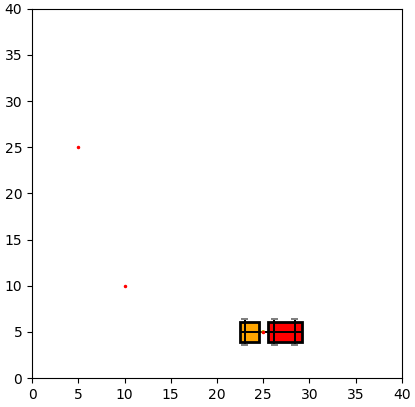
\includegraphics[width=0.45\textwidth]{images/pic1.png}%
        \label{fig:pic1a}%
        }%
    \hspace{0.5cm}%
    \subfloat[Situation after the first trailer facing]{%
        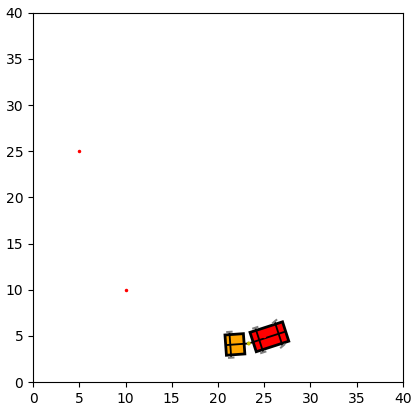
\includegraphics[width=0.45\textwidth]{images/pic2.png}%
        \label{fig:pic1b}%
        }%
    \caption{Trailer facing}
\end{figure}

In the picture above, we can see an example of the \emph{trailer facing} working. The initial conditions are the ones shown in \ref{fig:pic1a}, and our aim is to arrive to red point at (10, 10). If we were not using a trailer, we would steer the car such that it went towards higher $y$. However, as we can see in \ref{fig:pic1b} we are doing the exact opposite: we are going to even lower $y$. Once we have done this, the trailer is properly faced: when we go to the red point, the trailer will not jackknife as easily as if we had gone to the red point when we were in \ref{fig:pic1a}. This is because, when going to the red point, the trailer will bend to the opposite direction after the trailer facing, thus having to cross through the point $\phi = 0$.

However, we still have to decide what having a proper facing means. We will set a $\phi_{max}$ at which we end the trailer facing. This $\phi_{max}$ will not be static. If we are far away from the end point, we will set a high $\phi_{max}$, as we want to bend more. If we are close to the point, we will set a lower $\phi_{max}$, as we do not need to bend that much. In all cases, when $\phi = \phi_{max}$ we will end the trailer facing and start the car facing.\\


Once we have the trailer facing into the right direction, we start the second part of the manoeuvre: car facing. In this part, we act as if we had no trailer and we choose the $\delta$ such that the car goes to the end point. We do this until the trailer is faced into the wrong direction, and then we go back to the first part of the \textit{manoeuvre} again.\\

\begin{figure}[H] 
    \centering
    \subfloat[Faced trailer]{%
        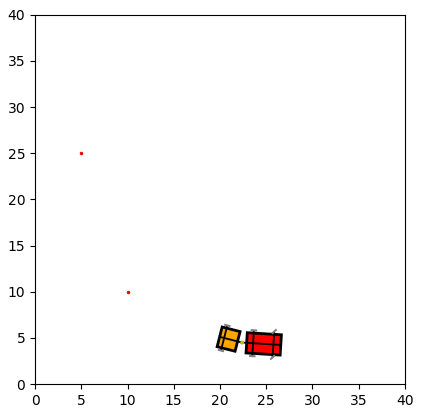
\includegraphics[width=0.30\textwidth]{images/picCF1.png}%
        \label{fig:piccf1a}%
        }%
    \subfloat[Trailer with $\phi \approx 0$]{%
        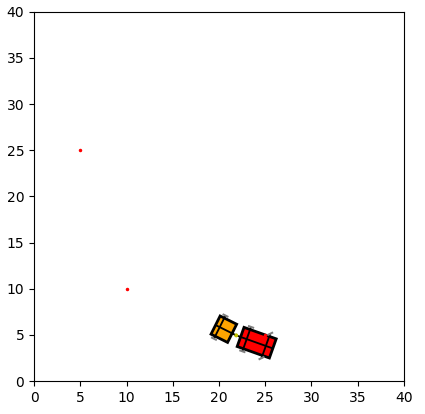
\includegraphics[width=0.30\textwidth]{images/picCF2.png}%
        \label{fig:piccf1b}%
        }%
    \subfloat[Trailer wrongly faced]{%
        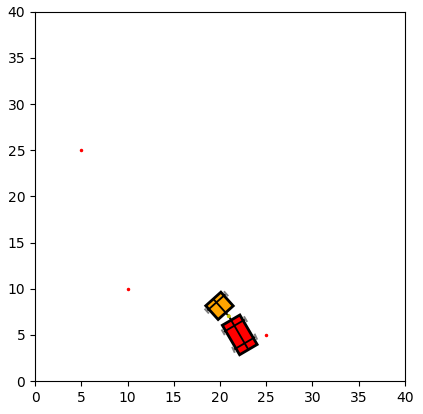
\includegraphics[width=0.30\textwidth]{images/picCF3.png}%
        \label{fig:piccf1c}%
        }%
    \caption{Trailer facing}
\end{figure}

In the picture shown above we can see how the trailer goes from being properly faced to a facing that if goes on it can cause a jackknife. In this picture we can see how the car gets closer to the red point ($y$ grows), and the price to pay is the misalignment of the trailer. Once it is enough misaligned, we will start with the trailer facing.\\

So far, we have just told about choosing $\delta > 0$ or $\delta < 0$, but we haven't specified which $\delta$ to use. In order to make the model more realistic, $\delta(t)$ will be a continuous function. That is, we are allowed a maximum variation of angle $\Delta \delta$ every time step $\Delta t$. That is, the maximum steering speed of the driver is $\Delta \delta / \Delta t$. For this reason, we can't always aim at the optimal $\delta$ every time step, as, if we were steering at $\delta_0$ at the last step, we can only aim at the best $\delta$ in $(\delta_0 -\Delta \delta, \delta_0 + \Delta \delta)$. How do we choose this best $\delta$? We use the discretised differential equation. Ideally, if we want to make an increase in $\phi$ of $\Delta \phi$, we have to take the $\delta$ satisfying the following equality:
\begin{align}
    \frac{\Delta \phi}{\Delta t} = - \frac{V}{L_{3}} \sin \phi - \frac{V}{L_{1}} \tan \delta \qty( 1 + \frac{L_{2}}{L_{3}} \cos \phi )
\end{align}
Which is given by:
\begin{align}
    \delta = \arctan\frac{-L1\cdot(\Delta \phi\cdot L3-\sin\phi\cdot\Delta t\cdot V)}{\Delta t\cdot V(L3+L2\cdot \cos\phi)} 
\end{align}
However, we cannot always choose this $\delta$, as this $\delta$ might not be in the interval $(\delta_0 -\Delta \delta, \delta_0 + \Delta \delta)$. For this reason, if $\delta > \delta_0 + \Delta \delta$, we choose $\delta = \delta_0 + \Delta \delta$. If $\delta < \delta_0 - \Delta \delta$, we choose $\delta = \delta_0 - \Delta \delta$.\\

Of course, we still need a criteria to decide which is the $\Delta \phi$ value that we want to attain. Different choices can be made, but we have chosen just to focus on the direction, not thinking about the actual value of $\phi$, for simplicity. If we want the trailer to go towards negative $\phi$ values, we will just set $\Delta \phi = -1$, and if we want it to go towards positive values we will choose $\Delta \phi = 1$. The decision of going towards positive and negative values is made upon the trailer facing or car facing criteria.



\subsection{Comparison of the two methods}

% As we have said before, the first method works by constantly looking for the optimal solution at the next time step. We have checked that this method does not work when aiming at a sufficiently large amount of time. The main drawback of this method is that the optimal configuration in the next step might not be good in the long run. On the other hand, the experienced method does not have this problem. Sometimes, it starts bending to the opposite side and getting much worse locally. However, this allows it to get better globally.

As we have said before, the first method works by constantly looking for the optimal solution at the next time step. We have checked that this method does not work when aiming at a sufficiently large amount of time. The main drawback of this method is that the optimal configuration in the next step might not be good in the long run. On the other hand, the steering-based method does not have this problem. Sometimes, it starts bending to the opposite side and getting much worse locally. However, this allows it to get better globally.



%---------------------The main drawback of this method is that the optimal configuration in the next step might not be good in the long run. On the other hand, the experienced method does not have this problem. Sometimes, it starts bending to the opposite side and getting much worse locally. However, this allows it to get better globally.--------------------------------------------
\subsection{Further improvements}

From experience, it is hard to make the trailer go straight, even when the axles are aligned (due to the fact that alignment is not perfect, and the equilibrium point is unstable). To model this, we can introduce some perturbations in the angle of the trailer. After doing an integration step, we will add some uniform noise to the $\phi$ angle, with expectation value $0$. We choose this kind of noise because a priori we do not have any preferred direction of the perturbations. The interval $(-r, r)$ of the uniform random variable that models the noise will have a fixed length $2r$, which has been chosen small (but way bigger than $10^{-16}$, which is the \textit{numerical noise} given by the finite decimals of the representation of the double precision numbers). The randomisation just affects to the kinematics, as the method to control the trailer is based on the same criteria. However, every trajectory of the trailer is different, due to the random effects. As, with $r = 0.025$, the trailer finishes successfully the path, this means that our method is robust and could be applied to ground with some slippery.\\

To illustrate that every simulation is different, and although the method is the same, it provides different steering functions $\delta(t)$, we have plotted in two runs of the method how $\phi$ and $\delta$ vary over time.

\begin{figure}[H] 
    \centering
    \subfloat[Comparison of $\phi(t)$ evolution]{%
        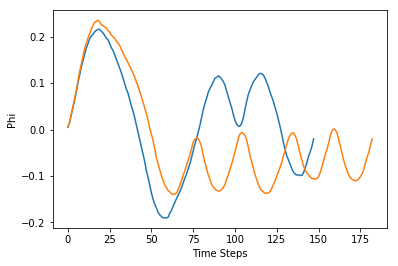
\includegraphics[width=0.45\textwidth]{images/phis.png}%
        \label{fig:phis}%
        }%
    \hspace{0.5cm}%
    \subfloat[Comparison of steering functions $\delta(t)$]{%
        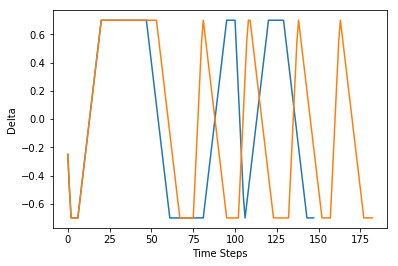
\includegraphics[width=0.45\textwidth]{images/deltas.png}%
        \label{fig:deltas}%
        }%
    \caption{Variation of the angles in different runs of the algorithm}
\end{figure}

We can see that one of the methods (blue) finishes earlier. Although having very different paths, they both terminate successfully. We can see that the initial conditions are similar but at some point they start to differ. After they start to differ, the steering functions change, as they adapt to the current $\phi$ value. As the steering starts to differ, this makes the path change more and more, ending with very different trajectories.